\chapter{Introduction}%
\label{chap:introduction}
\textit{This chapter narrows the broad field of robotics down to a largely unsolved problem, combining the three topics learning object dynamics, \ac{NAMO} and nonprehensile pushing. For that problem, the state-of-the-art methods are presented and their shortcomings are highlightedin the upcoming paragraphs. Then the gap in literature regarding the combination of the aforementioned topics is summarized in \Cref{sec:research_question} in the form of the main and sub research questions. The combination of the three topics is then narrowed down to the scope of this thesis in the problem description,~\Cref{sec:problem_description}. The chapter finishes by presenting all upcoming chapters in the report structure,~\Cref{sec:report_structure}.\bs}

% What's Purpose: The following issues are presented:
% - introduce 3 topics
% - joint-configuration space
% - multiple modes of dynamics, piecewise analytic
% - there are not much state-of-the-art, but these are them
% - backward search / backward induction

% What's Purpose: introduce 3 topics
\todo{MARTIJN: you introduce a lot of topics here, and make a lot of bold statements, all of which should be supported by relevant literature references.}
\todo{Martijn:  You should really structure your text so that you have one message per paragraph.}

For robots, it remains a hard problem to navigate and act in new, unseen environments. From the emerged challenges robots face in such envirionments, three topics are selected, namely: \textbf{learning object dynamics}, \textbf{\acf{NAMO}} and \textbf{nonprehensile pushing}. The main goal of this thesis is to combine these three topics, a secondary goal is to investigate how these topics can strengthen each other over time. When investigating the influence of the topics on each other, questions arise such as. How does learned environmental knowledge influence planning? Does the execution time decrease and how much for a repeated task? How much can generated action sequences improve as the robot learns more?\bs

Learning object dynamics enables the robot to manipulate unforeseen objects, \ac{NAMO} allows the robot to move around in an environment even if the robot's target location is blocked by an object, and nonprehensile pushing allows the robot to change the environment. Combining these 3 topics covers any task that involves relocating objects by pushing, which is a wide variety of tasks. Examples are clearing debris in construction sites or war zones or cleaning through pushing trash in one spot.\bs

\todo{maximal 2 examples per topic, --> ratjetoe}
Learning abilities allow robots to operate in completely new environments and improve robots to adapt to environmental changes. Such learning abilities are crucial when the robot can encounter many different objects. Examples are exploration or rescue missions in collapsed buildings, but also in more everyday robot applications. An unfamiliar environment can emerge from a familiar environment due to some unforeseen change that the robot is not aware of. An example is a leakage that changes the friction coefficient between the floor and everything standing on it. Another example are supermarkets, due to the presence of people in the supermarket the environment changes, providing a slightly new environment for the robots that operate in them.\bs

\todo{NAMO and nonprehensile pushing in some cases are the same, make a point that they are not becuase planning is required for the push}
\todo{NAMO should be here as you have learning above and pushing belwo}

Nonprehensile pushing is a form of manipulation that is widely available for robots, even though they are not intentionally designed for pushing. Mobile robots can drive (and thus push) against objects, and a robot arm with a gripper can push against objects even if the gripper is already full. Many robots can push, and pushing is a manipulation action many robots should leverage.\bs

\todo{Martijn(who is appeareantly not convinced)I am not convinced that you can really split all relevant research in these two categories, and they also don't sound like mutually exclusive categories.}
Research into approaches tackling the 3 topics just described can be split into two categories. The bulk falls into the category of hierarchical approaches~\cite{ellis_navigation_2022,krontiris_dealing_2015,scholz_navigation_2016,vega-brown_asymptotically_2020,wang_affordancebased_2020}. The remainder falls in category locally optimal approaches~\cite{novin_dynamic_2018,sabbaghnovin_optimal_2016,sabbaghnovin_model_2021}. Both approaches are elaborated upon later in this chapter. First, the configuration space is discussed that build up to the composite configuration space. Then second, two challenges are highlighted related to the composite configuration space growth of dimension and the fact that the composite configuration space is piecewise-analytic.\bs

% What's Purpose: composite configuration space
\paragraph{Configuration Space}
Now planning for a single action is investigated, and its relation to the configuration space. Finding a path for a single action (such as robot driving or robot pushing) is known as a \textit{motion-} or \textit{manipulation planning problem} and is planned in configuration space. \textit{Configuration space} for an object \gls{obj} can be described as an \gls{n_dof}-dimensional space, where \gls{n_dof} is the number of degrees of freedom for that single object \gls{obj}. A point in this \gls{n_dof}-dimensional configuration space fully describes where that object is in the workspace. Then the workspace obstacles are mapped to configuration space to indicate for which configurations the object \gls{obj} is in collision with an obstacle in the workspace. The subset of configurations in configuration space for which \gls{obj} is in collistion is called \textit{obstacle space}. The remainder of obstacle space subtracted from configuration space is free space, in which the object can move freely. For every object in the environment, a configuration space can be constructed. A mathematical description of configuration space can be found in \Cref{subsec:path_estimation}. When a configuration space is constructed, dedicated path planners leverage the configuration space to determine if a configuration lies in free or in obstacle space.\bs

\paragraph{Composite Configuration Space}
Now planning for an action sequence is investigated, and its relation to the composite configuration space. For a robot environment that involves relocating objects among the presence of other movable objects planning for a single action is not enough, because manipulating an object directly to a target position is in many cases, unfeasible. As a simple example, manipulating an object $\gls{obj}_A$ to a target position is feasible if the object, $\gls{obj}_B$ that blocks that path is first removed. Clearly, removing blocking object $\gls{obj}_B$ influences the feasibility of manipulating $\gls{obj}_A$ to its target position. For planning there must be a connection between the configuration space of $\gls{obj}_A$ and $\gls{obj}_B$, which is where the composite configuration space emerges. A \textit{composite configuration space} or composite space emerges when an objects configuration space is augmented with the configuration space of other objects~\cite{vandenberg_path_2009}. A composite configuration in such a composite space fully describes where the robot, and objects are in the workspace. In recent literature the composite configuration space is also named composite configuration space~\cite{vega-brown_asymptotically_2020}, finding \quotes{bridges} between configuration spaces~\cite{hauser_multimodal_2010} or room configuration~\cite{sabbaghnovin_model_2021}. The term composite configuration space has been selected because it indicates multiple configuration spaces composed together and does not confuse with joints (or hinges) of a robot. Path planners (in contrast to the planning in configuration space) have great difficulty to connect a starting composite configuration to a target composite configuration~\cite{roynicholas_hierarchy_2021} for reasons that are discussed in the upcoming paragraph.\bs

\paragraph{Challenges}
The first challenge with the composite configuration space is that is grows exponentially with the number of movable objects in the environment. An analysis is now provided with a robot environment in which both the robot and objects all have an two dimensional configuration space. The composite configuration space becomes $2(\gls{n_obj}+1)$-dimensional, with \gls{n_obj} is the number of objects in the environment. Thus the dimension of the composite space grows linearly with the number of objects in the robot environment, the composite configuration space itself grow exponentially, also known as the \textit{curse of dimensionality}.\bs

The second challenge is due to constraint sets, in configuration space a single constraint set applies. As an example, nonholonomic robots must respect a set of constraints due to the robots inability to drive in any direction. The class of robots that can be described by a bicycle model~\cite{polack_kinematic_2017} are nonholonomic. These robots cannot drive sideways, such as the boxer robot in \Cref{subfig:example_boxer_robot}. The nonholonomic constraints must be respected during planning, for the planner to yield feasible paths. In configuration space there exist only a single mode of dynamics~\cite{hauser_multimodal_2010}, and path planners such as \acs{PRM}~\cite{hsu_path_1997}, \acs{PRM*}, \acs{RRT} or \acs{RRT*}~\cite{karaman_samplingbased_2011} connect start to target configuration in configuration space whilst respecting the constraint set. In composite space there exist multiple modes of dynamics that must be respected. A drive action is connected to a different set of constraints than a push action. These different modes of dynamics make the composite configuration space \textit{piecewise-analytic}. Path planners have great difficulty crossing the boundary from one mode of dynamics to another mode of dynamics~\cite{vega-brown_asymptotically_2020}.\bs



% What's Purpose: multiple modes of dynamics, piecewise analytic
Finding an optimal solution to a \ac{NAMO} and pushing task requires a search in the composite configuration space. Apart from the fact that the composite configuration space becomes exponentially larger with every increase of objects, there is another problem.

\todo{Martijn: It doesn't make sense to me to suddenly talk about dynamics while everything else up to this point was quasistatic because you talked about configuration spaces and planning in those spaces.

Gijs introduce dynamics on top of planning}

\todo{Corrado: Cite roy, because When you say all this, you can easily refer to papers where they have the same definitions. I think nicoolas Roy uses this term a lot. It will make your claims and definition more robust. }

The composite configuration space is , which is explained below. Drive and push actions are translated to the composite configuration space as subspaces. A certain subspace of the composite configuration space is assigned to robot driving and another subspace is assigned to robot pushing. These different subspaces in composite configuration space are called different modes of dynamics. In the driving mode of dynamics, a set of driving constraints must be respected, and the pushing mode has a set of push constraints that must be respected. Such constraints originate from multiple sources, such as the robot being nonholonomic, the robots and objects properties (e.g.~geometry, weight distribution), friction coefficient between objects. Multiple modes of dynamics introduce a discontinuity in the constraints, hence the composite configuration space is a piecewise-analytic. 


Finding paths for multiple actions (such as first robot driving and then robot pushing) is known as multi-model planning~\cite{hauser_multimodal_2010} and is planned in composite configuration space. 


\Cref{chap:appendix_complexity_classes} contains an explanation on complexity classes which may be helpful to better understand this paragraph. As mentioned before finding an optimal solution to a \ac{NAMO} and pushing task requires a search in composite configuration space. Finding an optimal solution falls in category of \ac{NP-hard} problems, motivation is provided with the following simplification. If the search for an optimal solution in composite configuration space is simplified by completely removing relocating objects to new positions from the task, a purely \ac{NAMO} problem is what remains. If the problem is simplified even further, by assuming that every object is an unmovable obstacle, the problem falls in the category of \ac{NP-hard} problems because a reduction exists from the piano mover's problem which is known to be \ac{NP-hard}~\cite{reif_motion_1985}. That a simplified version is \ac{NP-hard} indicates how difficult it is to find an optimal path in composite configuration space.\bs

The last problem that is introduced is the uncertainty of actions in unknown environments. Planning an action sequence with limited or no environmental knowledge inevitably leads to unfeasible action sequences, such as pushing unmovable obstacles. Updating the environmental knowledge and replanning the action sequence is the cure to the uncertainty introduced by a lack of environmental knowledge. Trying to complete unfeasible action sequences is time and resources lost. Additionally, it can lead to the task itself becoming unfeasible. For example, a pushing robot ends up pushing an object into a dead end due to an action sequence planned with limited environment knowledge. Now that the object is in a stuck position the task has become unfeasible.\bs
\todo{Corrado: above and below could be the same paragraph}

tasks introduces a introduces a \ac{NP-hard} planning problem~\cite{wilfong_motion_1991}. Such an environment that consists of multiple objects


\todo{Corrado: talk about multi-modal planning}


To summarise, the main challenge is to \textit{find an action sequence for a given task to relocate objects that consist of push and drive actions in new and unforeseen environments}. To find such an action sequence a search cannot be performed in the composite configuration space because of two reasons. First the composite space grows exponentially with the number of movable objects. Secondly, the composite configuration space piecewise-analytic, path planners have great difficulty to cross boundaries from one mode of dyanamic to another. A multi-modal planning algorithm is sought, that can robustly find paths in composite configuration space, whilst avoiding the emerging challenges with composite space and handling the uncertainty introduced by the lack of environmental knowledge. A number of researchers tackled this problems. In the following we provide a categorization and a summary of the methods, advantages and disadvantages of the most relevant state-or-the-art methods.\bs








% What's Purpose: there are not much state-of-the-art methods, but these are them
\paragraph{Locally Optimal Approaches}
As has been indicated in the previous paragraph, finding a path in the composite configuration space cannot computationally be found in reasonable time (orders of magnitude slower than real-time, with no guarantees if no path exists). Only by leveraging simplifications applied to the composite configuration space, a search can be performed, such as considering a heavily simplified probabilistic environment~\cite{vandenberg_path_2009}, considering a single manipulation action~\cite{berenson_manipulation_2009}, discretization~\cite{sabbaghnovin_optimal_2016} or a heuristic function combined with a time horizon~\cite{sabbaghnovin_optimal_2016}. Such techniques prevent searching in configurations relatively far from the current configuration. Local optimality guarantees can be given and real-time implementations have been shown.\bs

\todo{Corrado: sabbagh has 3 papers, connect them: Corrado: Looks like 22, 23 and 18 are all connected. I miss to see the links, in the sense that the explanation is spread. Novin first started with 22 I guess, then built on topo of it in 18 and 23. But you start with 23. This requires better structuring }
\todo{Corrado: It would be nice to have a short overview of the whole method before diving into details later }
The most relevant locally optimal approach is presented by \citeauthor{sabbaghnovin_model_2021}~\cite{sabbaghnovin_model_2021}. She presents an optimal motion planner that avoids obstacles in the workspace and respects kinematic and dynamic constraints of a robot arm~\cite{sabbaghnovin_optimal_2016}. Examples of the motion planner are provided using a 3- and 4- \ac{DOF} planar robot arm. Sampling in the composite configuration space is simplified using discretization (by disjunctive programming) \todo{Corrado: cite disjunctive programming instead of throwing it in here} of the composite configuration space and by using a receding horizon. The disjunctive programming concept is applied for converting the continuous problem of path planning into a discrete form. In other words, a continuous path is made equivalent to some points with equal time distances which represent the entire path. After discretization the composite configuration space remains intracable. Thus a search is performed close to the current configuration by combining a heuristic function with a receding horizon concept. A specially developed heuristic function points \textit{toward} a target configuration, the planner then plans between the current configuration and a point toward the target configuration for a predetermined time horizon. The concept of a receding horizon is used to obtain the optimal path for every time step in the time horizon, but apply only the first term and repeating this process until the end-effector meets the final position.\bs

The optimal motion planner~\cite{sabbaghnovin_optimal_2016} is then converted toward path planning for a nonholonomic mobile robot with a gripper~\cite{novin_dynamic_2018}. With the 3-fingered gripper, the robot can grasp legged objects such as chairs or walkers. The targeted workspace is a hospital, where the robot is tasked with handing walkers (or other legged objects) to patients to lower the number of falling patients. The variety of legged objects motivates an object model learning module that learns dynamic parameters from experimental data with legged objects. The dynamic parameters are learned using a Bayesian regression model~\cite{scholz_navigation_2016}. An \ac{MPC} controller then tracks the path and compensates for modeling errors. A key contribution is that the planner can decide to re-grasp one of the object's legs to improve path tracking.\bs

Real world experiments show the effectiveness of Novin's locally optimal approach~\cite{sabbaghnovin_model_2021}. She has presented a manipulation planning framework focused on moving legged objects in which the robot has to choose between which leg to push or pull. The framework can operate in real-time, and the local optimality has been shown. From the 3 topics that this thesis focuses on, \citeauthor{sabbaghnovin_model_2021} includes learning object dynamics and prehensile manipulation of objects to target positions, missing only the \ac{NAMO} problem because a path is assumed to be free during object manipulation. Because Novin uses a gripper to manipulate objects, her research falls into the category of prehensile manipulation. Nonprehensile manipulation bears an additional challenge over prehensile manipulationthat is due to the contact points. With prehensile manipulation a gripper ensured multiple contact points, geometrically locking the object with respect to the gripper. The gripper and gripped object can be threated as a single object untill the gripper opens. With nonprehensile manipulation the object is not geometrically locked into place, adding an additional challenge for nonprehensile manipulation over prehensile manipulation.\bs.
\todo{check the last sentece above with chat u know what}

\paragraph{Hierarchical Approaches}
The second class of approaches to finding a path in composite configuration space is classified as hierarchical approaches~\cite{ellis_navigation_2022,krontiris_dealing_2015,scholz_navigation_2016,vega-brown_asymptotically_2020,wang_affordancebased_2020} that can be described as follows. A hierarchical structure generally consists of a high-level and a low-level component. The high-level task planner has an extended time horizon which includes several atomic actions and their sequencing. Whilst a low-level controller acts to complete a single action in a single mode of dynamics e.g.~drive toward object, push object. The high-level planner has a prediction horizon consisting of an action sequence, a long prediction horizon compared to the low-level planner whose prediction horizon is at most a single action.\bs

The most relevant hierarchical approach is presented by \citeauthor{scholz_navigation_2016}~\cite{scholz_navigation_2016}. He presents a planner for the \ac{NAMO} problem that can handle environments with under-specified object dynamics. The robot's workspace is split into various regions where the robot can move freely. Such regions can be connected if an object separating two regions and can be manipulated by the robot, to connect both regions. The manipulation action is uncertain because objects have constraints that the robot has to learn, e.g.~a table has a leg that only rotates, but cannot translate. A \ac{MDP} is chosen as a graph-based structure, where the nodes represent a free space region and objects separating the regions are edges in the \ac{MDP}. Finding a solution for the \ac{MDP}, leads to an action sequence consisting of a number of drive and object manipulation actions to eventually drive the robot toward a target position. The under-specified object dynamics introduce uncertainty in object manipulation. During action execution object constraints are captured with a physics-based reinforcement learning framework that results in improving manipulation planning when replanning is triggered.\bs

\citeauthor{scholz_navigation_2016} presented a \ac{NAMO} planner that makes use of a hierarchical \ac{MDP} combined with a learning framework, resulting in online learning of the under-specified object dynamics. The method's effectiveness in learning and driving toward a target location has been shown by an implementation on a real robot. From the 3 topics that this thesis focuses on, \citeauthor{scholz_navigation_2016} includes learning and the \ac{NAMO} problem, missing only push manipulation toward target locations. By not including manipulation of objects to target positions \citeauthor{scholz_navigation_2016} can find a global path without running into high dimensional spaces. In other words, by driving only the robot toward a target location a global path will encounter objects only once. By running into objects only once the manipulation of an object does not affect the feasibility of the global path, hence the simplification.\bs
\todo{Corrado: This is the same paper as above right? Why is there a blank line. Merge and avoid repetitions }

Both local optimal and hierarchical approaches have been discussed, both having their advantages and disadvantages. Local optimal approaches converge to a local optimal plan. To avoid the curse of dimensionality simplifications must be used to sample the composite configuration space in order to be computationally feasible. Such simplifications determine the quality of solutions found. Hierarchical structures generally provide solutions which are computationally efficient but are hierarchical, meaning the solutions found are the best feasible solutions in the task hierarchy they search. The quality of the solution depends on the hierarchy which is typically hand-coded and domain-specific~\cite{vega-brown_asymptotically_2020}.\bs

The most relevant work for local optimal~\cite{sabbaghnovin_model_2021} and hierarchical~\cite{scholz_navigation_2016} approaches are discussed. They both combine two of the three topics (one learning, and two \ac{NAMO} problem). Note both relevant works focus on prehensile manipulation, whilst this thesis focuses on nonprehensile push manipulation. Individually a considerable amount of research is done on these 3 topics (\ac{NAMO}~\cite{chen_fast_2018,elbanhawi_samplingbased_2014,ellis_navigation_2022,kingston_samplingbased_2018,lavalle_planning_2006,wang_affordancebased_2020}, nonprehensile push manipulation~\cite{arruda_uncertainty_2017,bauza_dataefficient_2018,mericli_pushmanipulation_2015,stuber_featurebased_2018,stuber_let_2020,toussaint_sequenceofconstraints_2022}, learning object dynamics~\cite{cong_selfadapting_2020,seegmiller_vehicle_2013}).
\todo{Martijn: YOU are repeating yourself, Corrado: agreed you repeat yourself}
Combining two topics received little attention by the scientific community and combining all three topics (to the best of my search) not at all. \Cref{table:sota_and_3_topics} presents state-of-the-art-literature and which portion of the three topics they include in their research.\bs

\todo{Martijn: Rightkmost column should be checks and marksa}
\todo{Choose: Specify object target positions or nonprehensile pushing}

\noindent
\begin{table}[H]
  \centering
  \rowcolors{2}{white}{myEvenLighterColor}
  \begin{tabular}
    {>{\raggedright\arraybackslash}P{2.5cm}%
      >{\raggedright\arraybackslash}P{2.0cm}%
      >{\centering\arraybackslash}P{1.4cm}%
      |>{\centering\arraybackslash}P{1.4cm}%
      >{\centering\arraybackslash}P{1.4cm}%
      |>{\centering\arraybackslash}P{1.4cm}%
      >{\centering\arraybackslash}P{1.4cm}
    }
    &&& \multicolumn{2}{c|}{\ac{NAMO}} & \multicolumn{2}{c}{\shortstack[c]{Specify object\\target positions}}\\
  Author&
  Citation&
  Learns\newline object\newline dynamics&
  \vspace{-0.2cm}\rotatebox{50}{prehesile}&
  \vspace{-0.4cm}\rotatebox{50}{nonprehesile}&
  \vspace{-0.2cm}\rotatebox{50}{prehesile}&
  \vspace{-0.4cm}\rotatebox{50}{nonprehesile}\\\hline
  \citeauthor{ellis_navigation_2022} &          \cite{ellis_navigation_2022} &          \cmark& \xmark& \cmark& \xmark& \xmark\\
  \citeauthor{sabbaghnovin_model_2021} &        \cite{sabbaghnovin_model_2021} &        \cmark& \cmark& \xmark& \cmark& \xmark\\
  \citeauthor{scholz_navigation_2016} &         \cite{scholz_navigation_2016} &         \cmark& \cmark& \xmark& \xmark& \xmark\\
  \citeauthor{vega-brown_asymptotically_2020} & \cite{vega-brown_asymptotically_2020} & \xmark& \cmark& \xmark& \cmark& \xmark\\
  \citeauthor{wang_affordancebased_2020} &      \cite{wang_affordancebased_2020} & \xmark& \xmark& \cmark& \xmark& \xmark\\
  Groote & Proposed Framework & \xmark/\cmark& \xmark& \cmark& \xmark& \cmark
\end{tabular}
\caption{Overview of 3 topics in recent literature and their object manipulation, where \textit{grasp-push} and \textit{grasp-pull} refer to prehensile push and pull manipulation, \textit{gripped} refers to fully gripping and lifting objects for manipulation, \textit{pushing} refers to nonprehensile push manipulation. The proposed framework shows \xmark/\cmark for learning system dynamics because it proposes system identification to generate a system model, however for the implementation an hardcoded system model is used.}%
\label{table:sota_and_3_topics}
\end{table}

\section{Research Question}%
\label{sec:research_question}
To investigate the effect of learning on action selection and action planning the following research questions have been selected.\bs

\textbf{Main research question:}
\begin{center}%
\label{researchquestion:main}
\large
How do learned objects' system models improve global task planning\\for a robot with nonprehensile push manipulation abilities over time?
\end{center}

The main research question is split into two smaller more detailed subquestions.\bs

\textbf{Research subquestion:}
\begin{enumerate}
    \item\label{researchsubquestion:does_it_work} How to combine learning and planning for push and drive applications?
    \item\label{researchsubquestion:does_it_compare} How do learning system models and remembering interactions compare to only learning system models? And, how does the proposed framework compare against the state-of-the-art?
\end{enumerate}

\textbf{The main contribution of this thesis is to combine all three topics.} These topics are learning object dynamics, the \ac{NAMO} problem and nonprehensile push manipulation. The proposed framework combines these 3 topics with the \textit{\acl{halgorithm}}. The algorithm builds a graph-based structure with nodes and edges, named the \textit{\acl{hgraph}}. Planning directly in the composite configuration space is avoided. The \acl{halgorithm} plans only in a single mode of dynamics and searches for a global path with a technique known as a backward search~\cite{krontiris_dealing_2015}. Learned object dynamics are stored in a knowledge base called the \textit{\acl{kgraph}}. The \ac{halgorithm}, \ac{hgraph} and \ac{kgraph} are introduced in \Cref{chap:hgraph_and_kgraph}.\bs

\section{Problem Description}%
\label{sec:problem_description}
To answer the research questions, tests are performed in a robot environment. A simple environment is desired because that simplifies testing, yet the robot environment should represent many real-world environments in which robots operate, thus a 3-dimensional environment is selected. The environment consists of a flat ground plane since many mobile robots operate in a workspace with a flat floor, such as a supermarket, warehouse or distribution center. An environment with a flat floor and a flat robot can be treated as a 2-dimensional problem because the robot and objects can only change position over \gls{x} and \gls{y} axis ($xy$ plane parallel to the ground plane) and rotate around the $z$ axis (perpendicular to the ground plane). A flat robot is selected because it has a low center of gravity, which lowers the chance of tipping over.\bs

Let's start with defining the environment. Let the tuple $\left\langle \gls{origin}, \gls{groundPlane}, \gls{Obj}, \gls{motionEquations} \right\rangle$ fully define a robot environment where:\bs

\noindent
\begin{table}[H]
\centering
\begin{tabular}
  {>{\raggedleft\arraybackslash}p{0.13\textwidth}%
  >{\raggedright\arraybackslash}p{0.77\textwidth}}
\gls{origin}& Static point in the environment with a $x$-, $y$- and $z$-axis. Any point in the environment has a linear and an angular position and velocity with respect to the origin \vspace{0.5\baselineskip}\\
\gls{groundPlane}& A flat plane parallel with the Origin's $x$- and $y$- axis. Objects cannot pass through the ground plane and meet sliding friction when sliding over the ground plane. \vspace{0.5\baselineskip}\\
\gls{Obj}& A set of objects, $\gls{Obj} = (ob_1, ob_2, ob_3, \dots, ob_i)$ with $i\geq1$, an object is a 3-dimensional body with shape, can be unmovable or movable. In the latter case, the mass is uniformly distributed. The robot itself is considered an object, an environment thus contains one or more objects. Examples of objects are given in \Cref{fig:example_objects}. \vspace{0.5\baselineskip}\\
\gls{motionEquations}& A set of motion equations describing the behavior of objects. \vspace{0.5\baselineskip}\\
\end{tabular}
\end{table}

A configuration consists of the linear position of an object's center of mass with respect to the environment's origin and the angular position of an object's orientation with respect to the environment's origin.\bs

Formally, a \textbf{configuration}, $c_{id}(k)$ is a tuple of $\left\langle pos_x(k), pos_y(k), pos_\theta(k)\right\rangle$ \quad where $pos_x, pos_y \in \mathbb{R}, \quad  pos_\theta \in [0, 2\pi)$ 

$k$ indicates the time step and can dropped to simplify the notation, \textit{id} is short for identifier and indicates the object to which this configuration belongs.\\

\todo{Gijs: you are a tennis ball, stay on a side, MARTIJN: I think that it is incomplete to talk about dynamic equations (in Eq) yet to ignore velocities here in your definition of the problem. In addition to configuration I think that you should talk about state (which encompasses configuration).}
\subsection{Task Specification}%
\label{subsec:task}
\todo{Corrado: This is a bit of a useless sentence if I may say. You can simplify a lot of things in your text by just going to the point without going around in circles. 

Just say, 

To answer the research questions, a number of tasks is designed}
The research questions investigates the effect of learning system models and monitor the effect of learned knowledge over time. Thus the robot needs an incentive to learn object properties, and interactions with the objects in its environment, otherwise it would simply remain standing still in its initial location. Therefore the robot is asked to complete a task. A task is defined as a subset of all objects with associated target configurations\bs
\[\text{task} = \left\langle Ob_{task}, C_{targets} \right\rangle\]


\todo{this suggest that only the first k objects, from Obj, can take part in the task. The way you write it here and in the previous page, it is not possible to skip ob1, and start assigning targes from ob2 onwards.}
\todo{Corrado: Ob task = set ofj , see feedback from corrado}
where $Ob_{task} = (ob_1, ob_2, ob_3, \dots, ob_k) \subset Ob$, $C_{target} = (c_1, c_2, c_3, \dots c_k)$ and $k>0$.\bs

A task is completed when the robot manages to push every object to its target configuration within a specified error margin.
\todo{Corrado: I hope you will write the exact equation for success later in the experimental section }

\subsection{Assumptions}%
\label{subsec:assumptions}
To simplify the pushing and learning problem, several assumptions are taken, which are listed below.\bs

\noindent
\centerline{\begin{minipage}{0.9\textwidth}
\begin{assumption*}%
\label{assumption:closed_world}
\textbf{Closed-World:} Objects are manipulated, directly or indirectly only by the robot. Objects cannot be manipulated by influences from outside the environment.
\end{assumption*}\bs

\begin{assumption*}%
\label{assumption:perfect_object_sensor}
\textbf{Perfect Object Sensor:} the robot has full access to the poses and geometry of all objects in the environment at all times.
\end{assumption*}\bs

\begin{assumption*}%
\label{assumption:order_does_not_matter}
\textbf{Tasks are Commutative:} Tasks consist of multiple objects with specified target positions. The order in which objects are pushed toward their target position is commutative.
\end{assumption*}\bs

\todo{Martijn: this sounds so ad-hoc. At the very least, you should check all simulation results afterward, to ensure that objects did not fall over. Here, you should mention that you will do those checks, and then in the results section you should report that all checks were positive.}
\begin{assumption*}%
\label{assumption:no_tipping}
\textbf{Objects do not tip over:} Movable objects slide if pushed.
\end{assumption*}\bs
\end{minipage}}

The assumptions taken serve to simplify the problem of task completion. Note that in \Cref{sec:future_work} insight is given to remove all assumptions. By removing assumptions completing tasks becomes a harder problem, but a more realistic problem closer to real-world applications.\bs

\todo{what is a zero velocity component?}
Assumptions might have certain implications, which are listed below. The \hyperref[assumption:closed_world]{\textbf{closed-world assumption}} implies that objects untouched by the robot and with zero velocity component remain at the same position. Completed subtasks are therefore assumed to be completed for all times after completion time.\bs

The \hyperref[assumption:perfect_object_sensor]{\textbf{perfect object sensor assumption}} simplifies a sensor setup, it prevents Lidar-, camera setups and tracking setups with aruco or other motion capture markers. The existence of a single perfect measurement wipes away the need to combine measurements from multiple sources with sensor fusion algorithms, such as Kalman filtering~\cite{verhaegen_filtering_2007}.\bs

Certain tasks are only feasible if performed in a certain order (e.g.~the Tower of Hanoi). The \hyperref[assumption:order_does_not_matter]{\textbf{tasks are commutative assumption}} allows focusing only on a single subtask since it does not affect the completion or feasibility of other subtasks.\bs

\todo{Corrado: Maybe the assumption should be that a 3d world can be represented as 2d. This connects with what Martijn commented earlier as well and would include objects not tipping over or be lifted from the ground }
The \hyperref[assumption:no_tipping]{\textbf{objects do not tip over assumption}} ensures that objects do not tip over and suddenly have vastly different dynamics. In practice, objects will not be higher than the minimum width of the object, and spheres are excluded from the environment. This experimental strategy seemed sufficient whilst running experiments but does not guarantee that objects do not tip over.

\subsection{An Example of Robots and Objects}
To get a sense of what the robots and the objects look like, see the two robots that are used during testing in \Cref{fig:example_robots}. And among many different objects, two example objects are displayed in \Cref{fig:example_objects}.

\begin{figure}[H]
    \centering
    \begin{subfigure}{.5\textwidth}
    \centering
    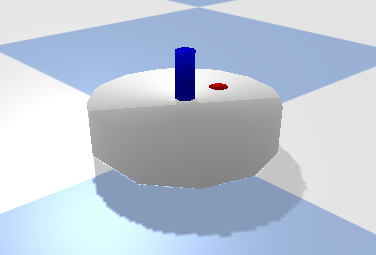
\includegraphics[width=0.8\textwidth]{figures/introduction/point_robot.png}
    \caption{The holonomic point robot the 2 velocity\\inputs drive the robot in \gls{x} and in \gls{y} direction}%
    \label{subfig:example_point_robot}
    \end{subfigure}%
    \begin{subfigure}{.5\textwidth}
    \centering
    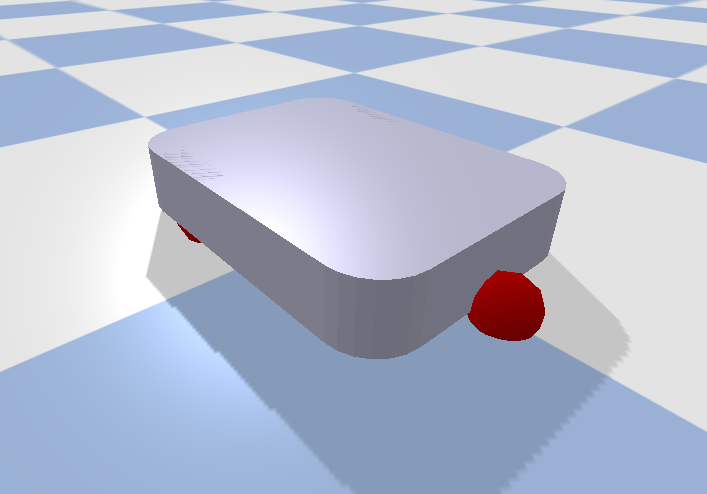
\includegraphics[width=0.8\textwidth]{figures/introduction/boxer_robot.png}
    \caption{The nonholonomic boxer robot, the\\input is forward and rotational velocity}%
    \label{subfig:example_boxer_robot}
    \end{subfigure}%
    \caption{Robots in the simulation environment}%
    \label{fig:example_robots}
\end{figure}

\begin{figure}[H]
    \centering
    \begin{subfigure}{.5\textwidth}
    \centering
    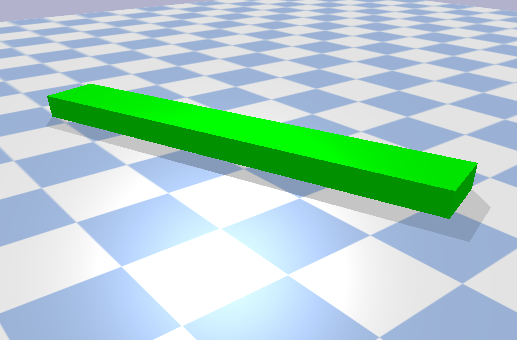
\includegraphics[width=0.8\textwidth]{figures/introduction/box_object.png}
    \caption{A box object}
    \end{subfigure}%
    \begin{subfigure}{.5\textwidth}
    \centering
    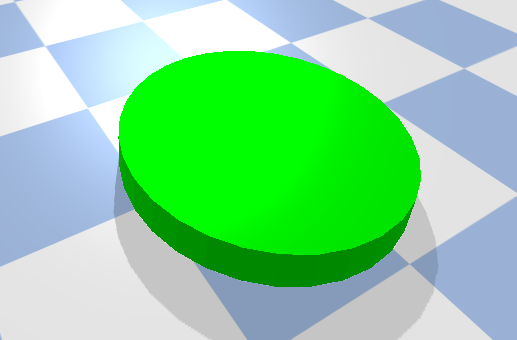
\includegraphics[width=0.8\textwidth]{figures/introduction/cylinder_object.png}
    \caption{A cylinder object}
    \end{subfigure}%
    \caption{Objects in the robot environment}%
    \label{fig:example_objects}
\end{figure}

For complete environments with accompanying tasks, see~\Cref{chap:results}.\bs

\section{Report Structure}%
\label{sec:report_structure}
\todo{Corrado: And the performance are tested in Chapter 4. 


Simplify the text to avoid repetitions and to shorten it}
The proposed framework heavily relies on a number of methods and functions. These methods and functions are conveniently grouped in \Cref{chap:required_background}. Then the proposed framework is presented and discussed in \Cref{chap:hgraph_and_kgraph}. Testing the proposed framework is presented in \Cref{chap:results}. The last chapter draws conclusions on tests and answering the research questions.\bs
